\documentclass{article}
\usepackage{graphicx}
\usepackage[francais]{babel}
\usepackage[T1]{fontenc}
\usepackage[utf8x]{inputenc}
\usepackage{amsmath}
\usepackage{amssymb}

\begin{document}

\begin{titlepage}
	\begin{center}
		\Large{Année universitaire 2016-2017}\\
		\Large{Université de Caen Basse-Normandie}\\[1cm]		
		\huge Rapport de Projet: Optimiseur de Wargame\\[0.5cm]
		\vspace{1cm}
		CANUET Maxime, CORBET Thorvald, JOLIVEL Valentin, L'HOMME Florentin\\
		\normalsize{\textit{ ~ L2 Informatique}}\\
		\vspace{2cm}
		
\includegraphics[scale=2.1]{../images/TRY1.png}
	\end{center}
\end{titlepage} 

\clearpage

\tableofcontents

\clearpage

\section{Présentation du jeu de Wargame}
 \subsection{Introduction}
 Dans le cadre du TPA, nous avons choisis le projet de l'optimiseur de wargame. Ce projet nous semblait être le plus intéressant. De plus ayant pratiqué de nombreux jeux de type \textit{"Wargame"} ou encore \textit{"Tactical RPG"} nous pensions avoir suffisamment d'expérience dans ce domaine.
 \subsection{Qu'est-ce qu'un Wargame?}
 Un Wargame est un jeu où le joueur est plongé dans une situation de conflit, une guerre, une escarmouche ou tout autre environnement se prêtant à des batailles. La célèbre série de jeu Starcraft est un bon exemple de Wargame. Pour notre projet nous avons décidé de réaliser un Wargame dans un monde avec un style Héroïque fantaisie.
 \subsection{Les règles du Wargame}
 Notre Wargame est un jeu de type tour par tour, la seule condition pour remporter la victoire est l'annihilation de l'équipe adverse (L'annihilation signifie que plus aucune unité adverse ne doit être présente sur le plateau de jeu). Chaque tour est divisé en deux phases bien distinctes. La première est la phase de déplacement. La seconde est la phase d'attaque. Pour de plus ample informations, consultez le livre de règles. Enfin chaque armée possède un nombre égal de points à répartir dans l'achat de ses unités (ce nombre est égal à 1000).
 
 \subsection{Comment jouer au Wargame}
 Notre Wargame est divisé en plusieurs phases que nous allons détailler ci-dessous.
 
 \subsubsection{Phase de préparation}
  Notre jeu est jouable en mode graphique. Pour pouvoir y jouer, lancez le fichier mainGUI.py. Une fois cela fait, cliquez sur le bouton "Jouer". Sélectionnez ensuite le type de joueur que vous désirez (Humain ou alors l'une des différentes IA proposées). Une fois cette action effectuée, si vous aviez décidé de jouer avec un joueur humain vous avez la possibilité de choisir son armée parmi celles présentées (Pour le moment, seul les Humains ainsi que les Orks possèdent des icônes pour leurs troupes). Dès que votre choix est fait, le jeu vous proposera de créer votre armée en choisissant parmi 7 unités différentes. Cliquez ensuite sur le bouton "Stop" pour lancer la partie.
  
  \subsubsection{Phase de jeu}
  Une fois votre armée prête, la phase de jeu débute. Comme nous l'avons dit précédemment, le jeu se déroule en tour par tour de ce fait le premier joueur commence par placer ses unités en cliquant sur la grille. Une sécurité est mise en place afin que le joueur ne puisse pas poster ses troupes n'importe où, la zone de départ étant de 4 cases de hauteur et aucune restriction sur la largeur. Une fois que les deux joueurs ont placé leurs troupes, la bataille peut commencer ! Pour cela les joueurs commencent par déplacer leurs troupes sur le terrain en cliquant sur l'unité qu'ils souhaitent déplacer puis sur la case de destination. Bien évidemment des mesures ont été prises pour cadrer les actions du joueurs, il ne peut par exemple pas déplacer une unité plus que ses points de déplacement ne le peuvent. Suit alors la phase d'attaque qui se déroule comme la phase de déplacement sauf que l'on ne clique pas sur une case vide mais une case contenant un ennemi. Un message sera affiché au joueur pour savoir si l'unité peut attaquer ou non (attaque déjà faite ou pas d'ennemis à portée). Une fois qu'une des deux équipes est complètement éliminées, un message de victoire apparait signalant le joueur vainqueur.

\section{La réalisation du jeu en mode console}
Après réflexion le groupe s'est accordé sur le fait de créer le jeu en mode console dans un premier temps.
En effet pour la réalisation de l'IA et pour le bon fonctionnement de l'algorithme génétique le jeu doit être parfaitement jouable en mode console.

 \subsection{Les plateaux}
 Dans notre jeu nous avons défini deux plateaux bien distinct. Un premier plateau dans lequel nous allons placer les unités des deux armées et un deuxième contenant l'environnement (Éléments naturels et constructions humaines). Ce second plateau ne contient actuellement que les valeurs 0 et 1 pouvant être respectivement traduite par "plaine" et "point d'eau", autrement dit une zone accessible aux unités et une zone non traversable. Une méthode de l'objet Plateau permet de générer une grille d'obstacles à partir de ces deux grilles (Notamment utilisée pour l'algorithme A*).
 
 \subsection{La création des unités}
 Dans un premier temps nous avons créé les unités dans un tableau pour pouvoir définir les statistiques de chacune d'elles et mettre en place un calcul de points (coût) par unité. Cette représentation sous forme de tableau nous donnait un bon aperçu des données de chaque armée. Nous avons donc pu, par exemple, équilibrer le prix des unités pour obtenir des armées assez équilibrées (En prenant en compte les spécificités de chacune, par exemple les Orks sont moins puissant mais plus nombreux).
 \begin{figure}
 \center
 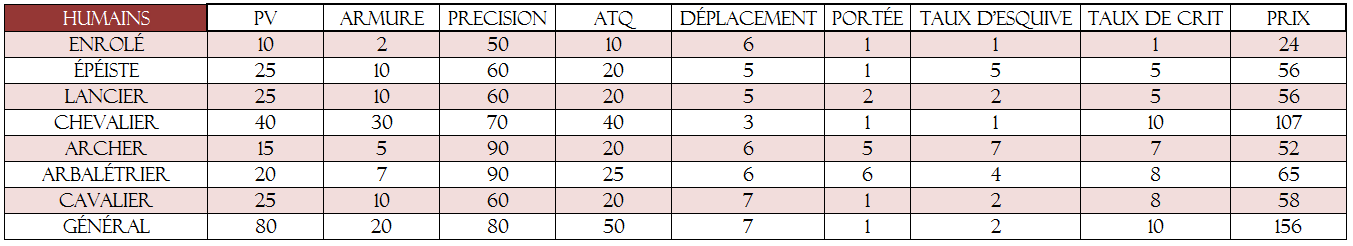
\includegraphics[scale=0.6]{../images/tableau.png}
 \caption{Exemple : Tableau des unités de l'armée "Humains"} 
 \end{figure}
 
  
  \subsubsection{Le calcul de points}
  Pour calculer le prix de chaque unités des différentes armées, nous nous sommes basé sur une formule prenant en compte toutes les statistiques. Ce calcul est le suivant: 
  
  \begin{flushleft}
   Prix: Potentiel offensif + Potentiel défensif + portée
  
  Potentiel offensif: [attaque*(precision+taux de critique+1)]/100
 
  Potentiel défensif: (PV+armure)+[(PV+armure)*taux d'esquive]/100
  
  portée: déplacement+portée
  \end{flushleft}
  
  \subsection{Le csv}
Nous avons utilisé le tableur pour entrer toutes les informations relatives aux statistiques des unités des différentes armées. Cependant, pour réutiliser ces données en python nous avons utilisé des fichiers .csv créés directement depuis le tableur. Cela permet une réutilisation simple des statistiques de base des unités, en allant chercher les informations dans le csv, et cela permet aussi de pouvoir modifier de façon claire les unités à partir du tableur (il suffit ensuite de produire de nouveaux fichiers .csv) tout en pouvant faire divers calculs sur ces statistiques. Les fichiers csv contiennent toutes les informations du tableur, les lignes les unes en dessous des autres et les colonnes séparées par des virgules. 
  
  \subsubsection{Les unités dans le programme}
  Les unités sont définies dans le fichier \textit{"unite.py"}. Dans la classe nommée \textit{"Unite"} on défini toutes les caractéristiques de chaque unité. En plus de cela, nous ajoutons ses coordonnées, la quantité de déplacement restante (En case) ainsi que le nombre d'attaques pouvant être encore effectuées. Les coordonnées renseignées permettent un déplacement simplifié mais permettent aussi de détecter plus rapidement l'ennemi le plus proche, ce en analysant les coordonnées des ennemis via la composition de l'armée plutôt qu'en analysant l'ensemble du plateau de jeu.
Nous avons ensuite créé une \textit{"factory"}. La \textit{"factory"} est une méthode abstraite qui crée une unité à partir de sa race et son nom en lui appliquant ses caractéristiques. Enfin la \textit{"factory"} est utilisée dans la fonction \textit{"addUnite"} pour pouvoir créer une armée et ce en tenant compte du solde de point encore restant.
  
 \subsection{La création des armées}
 Pour créer sont armé, le joueur doit cliquer sur les symboles "+" pour ajouter une unité et "-" pour la supprimer. Il répète cette action jusqu'à atteindre le seuil pré-fixé.
  
\subsection{Algorithme Astar}

	À de multiples reprises, cet algorithme se révèle très utile. Astar, permettant de trouver l'un des plus courts chemins entre un point D (départ) et un point A (arrivée), se voit utile tout d'abord en mode joueur humain. Le joueur cherchant à déplacer ses unités au travers de la carte, l'application se devait d'imposer un système "réaliste" de déplacement, c'est à dire sans traverser un obstacle tel qu'un point d'eau, une construction (Ex : une maison) ou encore des régiments ennemis (Traverser un régiment allié peut être toléré). En prenant en compte des obstacles, comme ceux précédemment cités, Astar renverra donc un chemin s'il en existe un. Il ne restera plus qu'à vérifier si l'unité que l'on souhaite déplacer possède assez de points de déplacements pour emprunter ce chemin.
	En plus du mode joueur humain, Astar trouve une grande utilité du côté du mode joueur IA jusqu'à en devenir presque indispensable. En effet, en mode joueur humain, nous aurions pu faire abstraction de cet algorithme en demandant simplement au joueur de "tracer" lui même le chemin à traverser, par la suite, il aurait été facile de vérifier la validité de ce chemin (Obstacles, longueur etc…). En mode joueur IA vient alors un problème : Comment faire en sorte que l'IA choisisse un chemin plus ou moins optimisé (Court et sans obstacles) ? Là intervient Astar, une fois choisi un point d'arrivée, l'algorithme rempli sa fonction en renvoyant un chemin allant des coordonnées initiales de l'unité jusqu'à sa destination. Contrairement au cas d'un joueur humain, nous ne sommes pas obligé de refuser un déplacement trop long proposé par Astar, au contraire, grâce aux coordonnées dans le plateau de jeu, on peut déterminer quelle unité ennemi est la plus proche (par exemple avec les distances de manhattan ou encore en lançant un Astar vers plusieurs unités ennemis) et prendre comme destination ses coordonnées. Si Astar renvoie un chemin, c'est qu'il en existe un jusqu'à la cible, on peut alors diriger notre unité vers celle-ci en parcourant, même partiellement, le chemin obtenu via l'algorithme. En d'autres mots, les déplacements d'un joueur IA repose essentiellement sur l'Algorithme Astar.

 \subsubsection{Pré-requis}

	L’exécution de l'Algorithme Astar nécessite bien évidemment quelques pré-requis (arguments à renseigner dans l'appel de la fonction), de façon évidente les coordonnées initiales et les coordonnées finales espérées ainsi qu'une grille composée uniquement de 0 (Obstacles) et de 1 (Cases libres). Le plateau de jeu ne peut donc être fourni de façon brut, il faudra alors dans un premier temps réaliser une grille correspondante à l'analyse de notre plateau de jeu, ceci étant réalisable via la méthode grilleObstacle de l'objet Plateau. Optionnellement, nous pouvons indiquer à Astar la liste des directions dans lesquelles le déplacement est possible, par défaut direction = [(1,0), (-1,0), (0,1), (0,-1)] soit "Droite", "Gauche", "Bas" et "Haut".

  \subsubsection{Principes de l'algorithme et heuristique choisie}

	Initialement, Astar commence par les coordonnées de départ renseignées. À partir de celles-ci, on analyse les successeurs possibles, autrement dit les cases vers lesquelles nous pouvons nous diriger. On attribue alors à ces cases une heuristique, un coût théorique/estimé depuis le point de départ jusqu'à l'arrivée. L'heuristique choisie correspond au nombre de déplacements effectués depuis le départ + la distance de manhattan entre la position actuelle et l'arrivée. Dans l'exemple ci-dessous, chacune des cases en cours d'analyse (Première image à gauche) ont effectué 1 déplacement et + 5 de distance de manhattan pour celles situées en haut et à droite ou + 7 pour celles situées en bas et à gauche. Deux des cases ont donc une heuristique égale à 6, les deux autres égale à 8.
	
  \begin{figure}[h]
	\center
	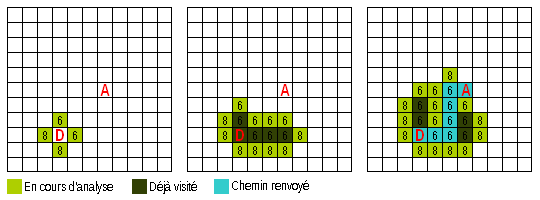
\includegraphics[scale=1.2]{../images/Astar01.png}
  \end{figure}

	On continue alors l'algorithme en prenant la ou l'une des heuristiques les plus faible, notre but étant de trouver un chemin court de préférence. On prendra donc ici l'une des cases d'heuristique 6, on analyse ensuite les successeurs possibles non visités, la case de départ étant notre point d'origine fait donc évidemment parti des cases déjà visitées. On calcule les heuristiques de ces successeurs et on recommence en prenant l'une des cases avec le minimum d'heuristique, ce jusqu'à parvenir au point d'arrivée ou, dans le cas contraire, ne plus avoir de cases à visiter. Une fois terminé, Astar renvoie une liste de coordonnées s'il trouve un chemin valide entre le départ et l'arrivée, s'il ne trouve pas de chemin, il renvoie False.

  \begin{figure}[h]
	\center
	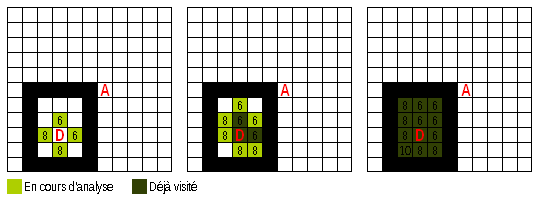
\includegraphics[scale=1.2]{../images/Astar02.png}
  \end{figure}
	
	Pour obtenir de bons résultats avec Astar, il est nécessaire de choisir une bonne heuristique. Pour le schéma présenté ci-dessous, le chemin jaune est le plus court des deux présentés, au centre se trouve le résultat obtenu avec une mauvaise heuristique, à droite celle semblant être la meilleure et, accessoirement, étant celle que nous avons retenu. Au centre, l'heuristique correspond à la somme de l'heuristique précédente (0 pour le point de départ) + 1 (Le déplacement) + la distance de manhattan jusqu'à l'arrivée, avec cette heuristique, nous n'obtenons visiblement pas le meilleur résultat. A droite, l'heuristique correspond à la somme de la distance parcourue depuis le point de départ (Distance réelle et non de manhattan) + la distance de manhattan jusqu'à l'arrivée.

  \begin{figure}[h]
	\center
	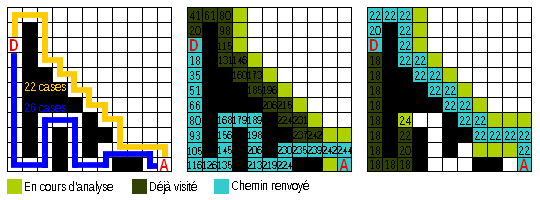
\includegraphics[scale=1.2]{../images/Astar03.png}
  \end{figure}

 
 \subsection{Le déplacement des armées}
 Le déplacement des armées se fait unité par unité. Notre fonction \textit{"deplacementArmee"} permet au joueur d'entrer la case sur laquelle l'unité veut se déplacer. Elle vérifie ensuite si cette case est contenue dans la zone de déplacement possible. Enfin, elle vérifie que la case soit vide pour ensuite pouvoir effectuer le déplacement.
 \subsection{la phase d'attaque}
 La phase d'attaque est permise aux unités qui ont au moins un ennemi à portée. La fonction qui s'occupe de l'attaque pour un joueur humain se nomme "attaquer", celle-ci fait appel à d'autres fonctions comme \textit{"testPrecision"} qui va déterminer si l'unité réussi son attaque, une autre permet de tester si l'ennemi esquive le coup, une autre encore supprime des points vie à une unité touchée.
 
\section{Les Intelligences artificielle}
 Nous voulons proposer différentes IA pour permettre aux joueurs d'éprouver leurs facultés de stratèges contre des IA plus ou moins intelligentes. Pour la première partie de notre projet nous nous somme contentés de deux IA. Une première, qui laisse découvrir aux joueurs les mécanismes du jeu. Et une seconde, permettant aux joueurs de jouer pour se détendre. Ces deux IA sont prévues pour nous donner une base et permettre aux joueurs de s'habituer au jeu. Par la suite nous voudrions développer une IA capable de donner du fil à retordre aux utilisateurs. 
 \subsection{L'IA simple}
  L'IA simple est une IA très rudimentaire. Elle sert de base pour les autres IA (Elle sera aussi utilisée dans l'algorithme génétique à titre d'exemple, mais pas pour obtenir une véritable armée optimisée). Comme les autres IA, celle-ci possède son propre fichier permettant de la sélectionner pour le déroulement d'un combat. Nous allons vous détailler son fonctionnement.
  
  \subsubsection{La création d'armée via l'IA}
  L'IA simple se contente d'aller rechercher des armées pré-faites dans un fichier csv. L'IA va chercher la race ainsi que la composition d'une armée pré-enregistrée dans le csv.

  \subsubsection{Le placement des unités}
 Cette IA place ses unités de manière aléatoire sur le plateau en respectant la zone de placement. Pour chaque unité, elle vérifie la validité du positionnement, autrement dit elle vérifie que les coordonnées choisies ne correspondantes ni à une unité déjà placées ni à un obstacle naturel. Si les conditions sont respectées, l'unité est placée, sinon de nouvelles coordonnées sont (re)tirées aléatoirement. 
 
  \subsubsection{Le déplacement}
 Cette IA se déplace de manière aléatoire sur le plateau et attaque si un ennemi se trouve à portée. Son fonctionnement est relativement simple, en effet on parcourt la liste des unités de notre armée puis on parcourt celle de l'ennemi. Les unités potentiellement attaquable sont placées dans une liste qui sera utilisée pour l'attaque. Si la liste est vide, on crée une liste dans laquelle seront mises les cases possible pour le déplacement de l'unité. Enfin, le déplacement est choisis au hasard dans cette dernière liste.
 
  \subsubsection{Les attaques} 
 La fonction d'attaque pour l'IA reprend le même principe que la fonction d'attaque pour un joueur humain à ceci près que, si l'unité de l'IA a à portée plusieurs unités ennemis, elle se dirige vers le plus proche. 
 
 \subsection{L'IA médium}
 Cette IA est encore en développement, elle aura des déplacements rudimentaires. En effet chaque unité se déplacera vers l'unité ennemie la plus proche.
 
\section{L'optimiseur}

	\subsection{Algorithme Génétique}
		Le principe de l'Algorithme Génétique est de tourner sur plusieurs générations afin de garder les éléments les mieux adaptés à une situation.
		
		Par exemple, prenons une population équilibrée de gazelle et de guépard. Petit à petit les gazelles vont se faire manger par les guépards. Par conséquent, même si dans de rares cas un guépard se fait tuer par les gazelles, la population va tendre vers une population uniforme de guépard. A la génération 0, il y aurait donc par exemple 50 guépards et 50 gazelles. Un affrontement a lieu entre les deux espèces, 20 gazelles et 2 guépards meurent. Entre les générations 0 et 1, des mutations et des croisements ont lieu entre les guépards, certains obtiennent donc un nouveau gène leur conférant une plus grande résistance à la faim, on les appellera les F-guépards. On arrive alors à la génération 1 actuellement composée de 48 guépards et 30 gazelles. Un affrontement a lieu, ne faisant que 5 victimes chez les gazelles. Ayant eu peu de nourriture, certains guépards meurent de faim, les F-guépards et d'autres guépards (normaux) s'en sorte bien face à cette pénurie. De nouvelles mutations et nouveaux croisements ont lieu, un gène R apparait, celui-ci confère une plus grande rapidité, les guépards le possédant pourront donc atteindre une proie plus facilement. A la génération 2, nous avons donc des guépards (normaux), des F-guépards, des R-guépards (rapide) voire des F-R-guépards (rapide et résistant à la faim), plus globalement on a 35 guépards et 25 gazelles. Un affrontement a lieu entre les deux populations, les (F-)R-guépards capturent la plupart des proies, les autres étant prises par les F-guépards plus en forme que les guépards normaux. A ce moment, toutes les gazelles ont péri, les guépards normaux, n'ayant toujours pas eu (ou peu) de nourriture, meurent aussi. Seul les F-guépards, R-guépards et F-R-guépards ont "survécu" jusqu'à la "fin" faisant d'eux les éléments les plus adaptés à la situation.
		
		Notre algorithme génétique fonctionnera (puisqu'il n'est pas encore opérationnel) de façon générale, c'est à dire, en reprenant l'exemple précédent par exemple, en ayant besoin de renseigner une population de départ, une fonction de sélection, une fonction de mutation et une fonction de croisement. Dans notre cas (le Wargame), la population de départ correspond à un ensemble d'armées. La fonction de sélection met en place des combats entre ces armées, les meilleures seront susceptible d'être présentes à la génération suivante, pour cela nous avons donc créé un système de tournois qui permet de sélectionner de façon assez juste les armées potentiellement les mieux optimisées. Les fonctions de mutations et de croisements seront implémentées ultérieurement, comme on peut le comprendre dans l'exemple précédent, ces dernières peuvent s'avérer cruciale dans cette optimisation.

	\subsection{Les tournois}
		Le système de tournois mis en place est relativement simple. Une population d'armée est renseignée à la fonction donc, pour une population de \textit{N} armées, il y aura (\textit{N}²-\textit{N})/2 combats différents (Combat avec soi-même exclu). Chaque cas est réalisé par une simple double-boucle. Néanmoins, le hasard peut parfois grandement intervertir le résultat d'un combat, pour éviter donc ces cas, un combat entre une armée \textit{$\textrm{N}_\textrm{1}$} et une armée \textit{\textit{$\textrm{N}_\textrm{2}$}} est rejoué plusieurs fois, celle qui remporte le plus de victoires est donc considérée comme la gagnante de l'affrontement. Les victoires des affrontements sont ensuite comptabilisées ce qui, à la fin, génère un classement. Il ne reste plus qu'à sélectionner un certain nombre d'armées parmi les plus fortes pour continuer dans l'algorithme génétique.

\section{La réalisation du jeu en mode graphique}
	La partie graphique du jeu a été réalisé avec Pygame. Le mode graphique se découpe en deux parties, la première partie est le fichier mainGUI.py, c'est ce fichier qu'il faut ouvrir pour lancer le jeux en mode graphique. Ce fichier contient peu de choses, il permet juste le lancement des fonctions permettant l'affichage des fenêtres de jeux. La seconde partie est le fichier GUIfunc.py, c'est ce fichier qui est le cœur du mode graphique, chacune des fonctions de ce fichier représente une fenêtre du jeux.
	
 \subsection{La charte graphique}
		Les couleurs choisies sont principalement le bleu et l'or, le mariage de ces deux couleurs rappellent la royauté afin de montrer que les combats menés par le joueur ne sont pas de simples batailles de campagne mais bel et bien des guerres menées par de puissants seigneurs. Ce choix de couleurs permet aussi un habillage sobre et efficace, ainsi on évite de surcharger l'interface et de perdre le joueur avec des couleurs dans tous les sens sans liens entre elles. Le choix d'une interface simpliste est fait pour mettre en évidence les éléments principaux de la fenêtre, la couleur "gris clair" permet notamment de créer un contraste entre le voyant de l'or qui est renforcé par le sombre du bleu à l'intérieur. La police choisie est "War of Asgard", c'est une police de style médiévale qui reste cependant très lisible de par le fait que les caractères ne sont pas tassés et que le dessin est suffisamment épuré pour ne pas ressembler à un amas de lettres. Le style médiévale de cette police a été choisi pour correspondre au thème de notre jeu qui est l'héroïque fantaisie. Les icônes représentant les unités sont pour le moment à l'état d'ébauche, pour ces dernières nous avons demandé l'aide de Morgane Jolivel, une jeune dessinatrice, afin d'obtenir un rendu à la fois cohérent (Plutôt que des images piochées par ci par là avec des styles graphique différents) et répondant à nos demandes, donc une images spécifique à chacune des unités (Et donc éviter de prendre quelque chose "à peu près ressemblant"). Cette association nous permet ainsi, en plus du travail de groupe, d'apporter un côté "Travail avec un/e groupe/personne tierce". Pour les musiques, nous utiliserons des musiques libre de droits ou bien comme pour les icônes nous les créeront nous même afin d'éviter tout problème de droits.
		
 \subsection{Préparation du combat }
		Sur cet écran se déroule le choix des joueurs, il y a au total deux choix principaux. Le premier choix est le joueur humain, dans ce cas des questions lui seront posées afin de savoir ses actions dans le jeu. Le second choix est celui de l'intelligence artificielle, ce choix se découpe sous trois catégories: simple, médium, difficile. Une fois que les deux joueurs sont choisis, on passe au choix de la race de son armée. Cet écran apparait seulement si un joueur humain est sélectionné, l'Intelligence Artificielle choisie elle-même sa race ainsi que la composition de son armée.
		
	\begin{figure}[h]
	\center
	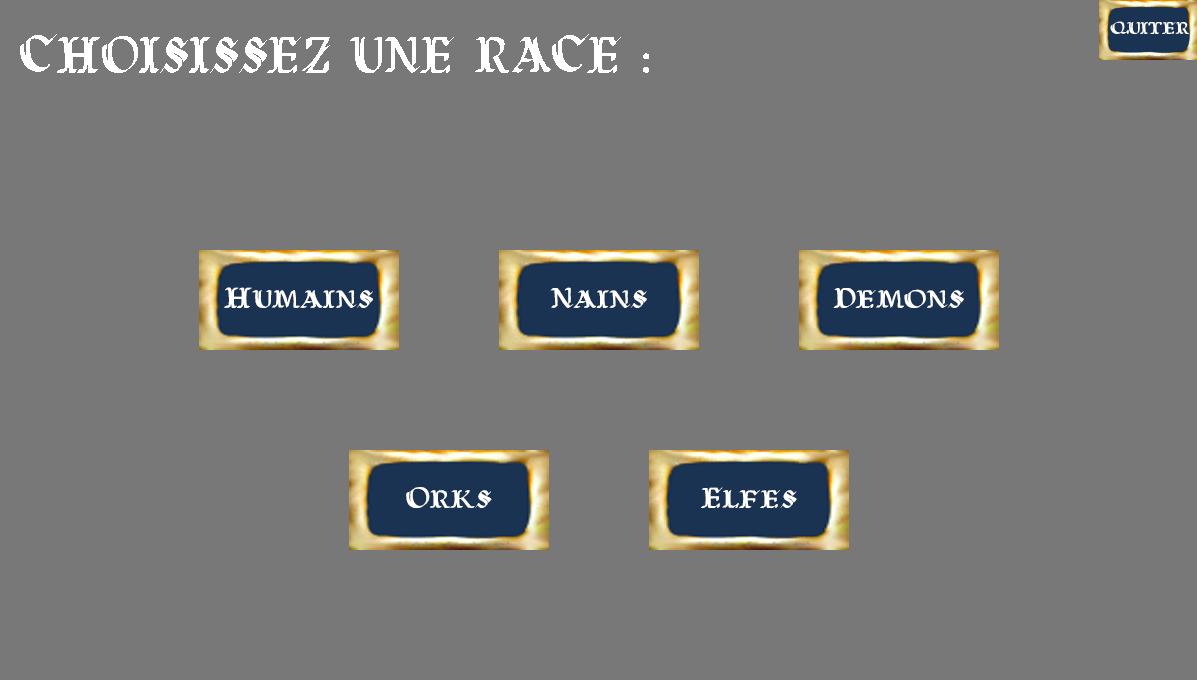
\includegraphics[scale=0.15]{../images/GUIraces.png}
  	\end{figure}
		
		Dans ces deux fenêtres, l'utilisateur aura simplement besoin de cliquer sur l'une des boites pour valider son choix. La simplicité de ces fenêtres est voulue car ainsi le joueur n'est pas perdu parmi un choix trop vaste. Ainsi les choix de ces paramètres se font de façon fluide.
		
  \subsubsection{Explication du code }		
		Ces deux fenêtres font parties des plus simples au niveau du code, elles ont toutes les deux une structure générale plus ou moins identique. En premier lieu on créé une variable vide qui contiendra les éléments à renvoyer pour la suite du programme. Ensuite on charge les images qui serviront de boutons pour l'utilisateur, on créé les événements liés au clic de la souris sur les images que l'ont a chargé précédemment, puis pour finir on réalise un test pour savoir si toutes les conditions sont réunies pour passer à l'écran suivant et on retourne les valeurs de la variable créée au départ dans le programme principal pour la traiter et passer à la suite du programme.
		
		def fenêtre(écran: "écran pour l'afficher"):
			
			variable = valeur à récupérer
			img = créerImage(chemin,nom)
			positionner image 
			
			si clique sur image:
				mettre nom image dans variable 
			
			si condition réunis :
				retourner variable
				
 \subsection{Phase de création de son armée }
		Une fois que l'utilisateur a choisi sa race, on passe sur l'écran de création des armés. Cet écran se divise en trois colonnes, dans la première colonne est affiché le nom des unités que le joueur peut acheter avec ses points ainsi que leur prix. La deuxième colonne est composée de trois éléments. Deux boutons, un bouton plus et un bouton moins, ils permettent d'ajouter et d'enlever des unités à la composition de l'armée, le dernier élément représente combien de fois cette unité est présente dans l'armée du joueur. La dernière partie de la fenêtre montre le solde restant du joueur, ainsi il pourra optimiser au mieux la composition de son armée par rapport à son solde. Une fois que le joueur aura terminé de choisir la composition de son armée, il lui suffira de cliquer sur le bouton stop.
		
	\begin{figure}[h]
	\center
	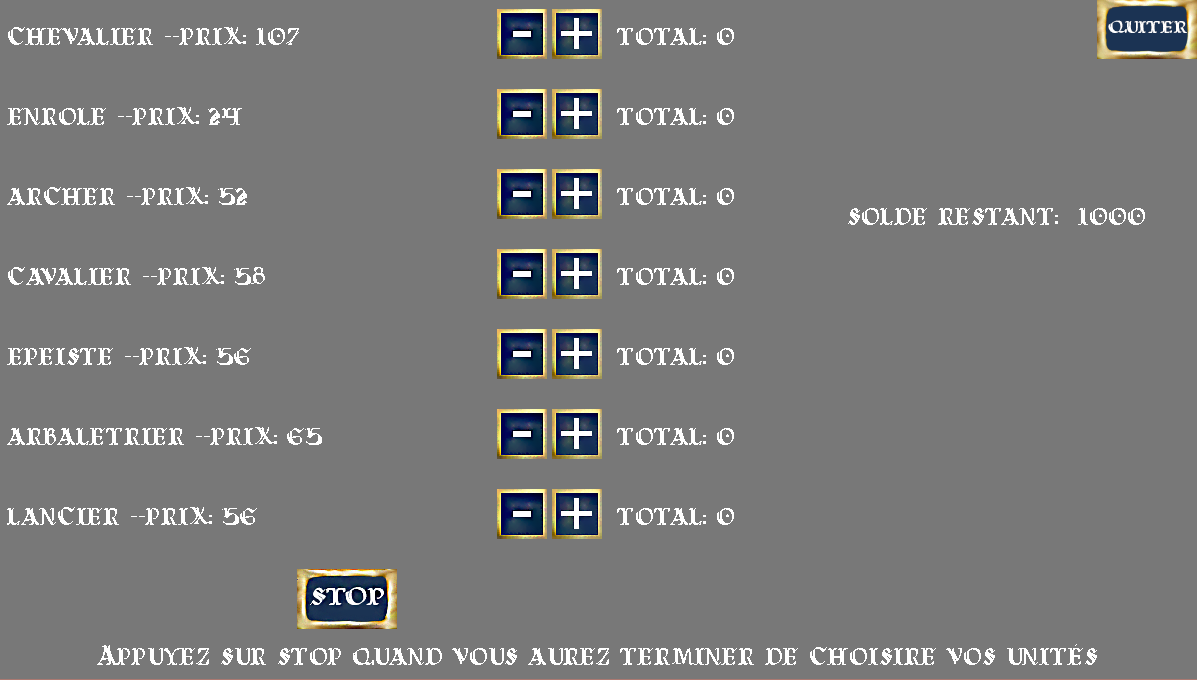
\includegraphics[scale=0.15]{../images/GUIcompo.png}
  	\end{figure}

		Le code de cette fenêtre est très ressemblant à celui des fenêtres précédentes à la différence que l'on ajoute une instruction pour compter les unités et le solde restant.
		
 \subsection{Phase de jeux: }
	Comme indiqué dans les règles le jeux se passe en tour par tour avec une phase de déplacement et une phase d'attaque. Le jeux se fera sur cette fenêtre.
	
	\begin{figure}[h]
     \center
      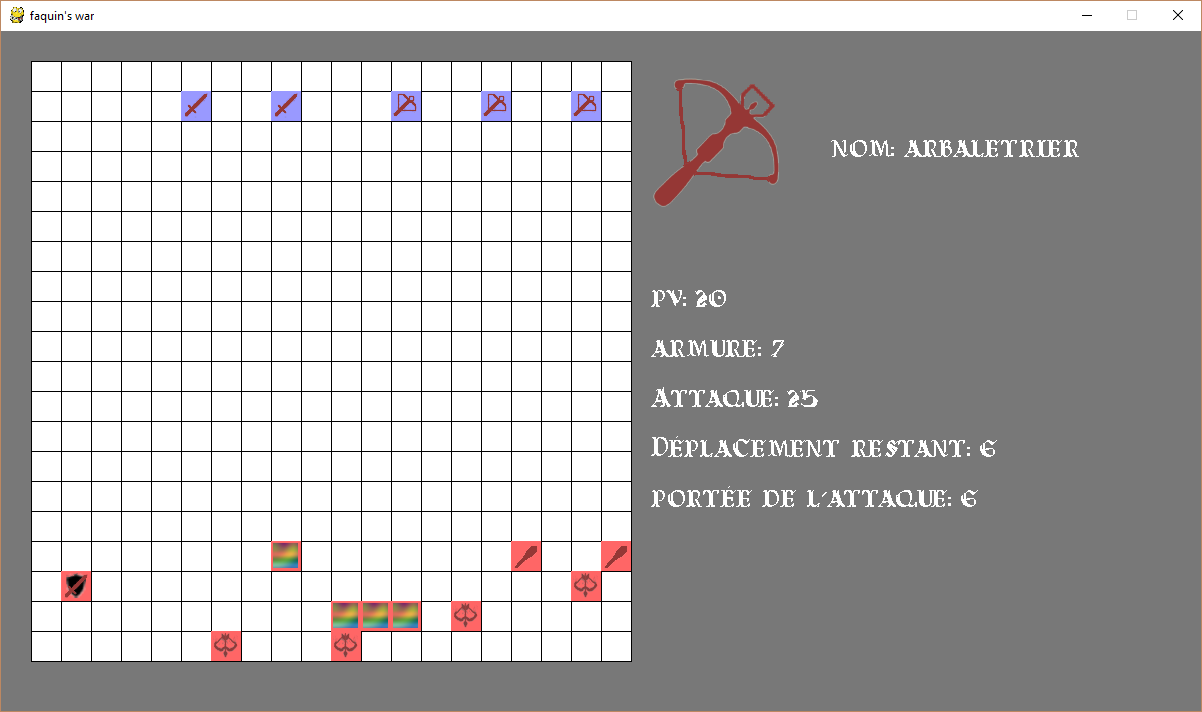
\includegraphics[scale=0.2]{../images/main.PNG}
     \caption{écran de jeu principal}
    \end{figure}
    	
	
	
	Cette fenêtre est scindée en deux partie, la première avec le plateau de jeu, c'est sur celle-ci que le joueur cliquera pour sélectionner  l'unité avec laquelle il fera son action. La seconde partie est là pour donner les informations sur l'unité qui a été sélectionnée, on retrouve sur cette partie les statistiques principales de l'unité, ainsi que son nom et une image la représentant (Identique à l'icône).
	
  \subsubsection{Explication du code }
	Pour cette partie, on divise le code en 5 fonctions distinctes. La première sert à créer la grille et afficher les pions sur cette dernière, pour cela on demande en entrée la liste des unités, ensuite on parcourt cette dernière en regardant les coordonnées de chaque unités puis on la place dans la grille réservée au placement des unités. En même temps, on converti les coordonnées de l'unité en pixel pour placer le pion sur la fenêtre après avoir préalablement dessiné la grille.
	
	La seconde fonction est celle qui permet de placer les pions au début de la partie. Pour cela on donne la liste des unités du joueur qui doit placer ses pions. Puis on demande au joueur de cliquer sur la grille à l'endroit où il désire placer son pion. Bien évidemment on fait des tests sur l'endroit cliqué par le joueur pour savoir si : Il clique bien sur la grille et si il est bien dans sa zone de placement. A chaque fois que le joueur clique sur une case autorisée, on fait appel à la fonction qui affiche les pions sur la grille cependant si le joueur clique sur une case non autorisée, un message d'erreur apparait sur l'écran lui en informant.
	
	La troisième fonction sert à créer l'affichage sur la partie droite de l'écran. Pour cela il nous faut deux paramètres, la race et le nom de l'unité. Ainsi on récupère précisément l'unité désirée dans un dictionnaire contenant les unités de chacune des deux armées, on récupère les statistiques désirées de cette unité puis on les affiche sur la partie droite de l'écran.
	
	La quatrième fonction est la fonction de déplacement. Cette fonction permet au joueur de déplacer ses pions durant la phase de déplacement, celle-ci diffère de la phase de placement par le fait que le joueur est libre d'aller où il veut sur la grille du moment que sa destination finale n'est pas une case où une unité ennemie est déjà présente ou un obstacle. Durant cette phase le joueur peut choisir quelle unité il veut bouger en premier, il lui suffit de cliquer dessus. Puis il lui suffit de cliquer sur la case où il veut aller, bien évidement des tests sont effectués pour valider ou non son choix.
	
	La cinquième fonction est la fonction permettant d'attaquer une unité ennemie, pour le moment cette fonction est encore à l'état d'ébauche. Cette fonction n'étant pas implémentée, sa description sera très sommaire. Pour cette fonction on donne les unités présentes sur le plateau puis comme pour la phase de déplacement, on clique sur notre unité attaquante puis sur l'unité qui sera attaquée.

\section{État du projet pour le semestre 1}
 \subsection{Travail réalisé}
Le jeu est jouable en mode console, et bientôt jouable en mode graphique. 
 \subsection{Travail à réaliser}
 Pour le second semestre nous devons terminer le mode graphique dans un premier temps (Les détails technique seulement). Ensuite nous allons travailler sur des IA plus poussées que nous utiliserons pour l'algorithme génétique sur lequel nous allons travailler. De plus nous enrichirons le jeu en ajoutant certaines spécificités telles que des bonus procurés par les généraux, des bonus/malus de dégâts lors d'une attaque en fonction des types des unités attaquante et défenseur etc...

\section{Conclusion}
 Pour le premier semestre nous voulions que le jeu soit jouable en mode console et qu'une base pour les IA développée soit créée. Ces objectifs ont été atteint et une version graphique est en cours de développement. Toutes les bases de notre projet sont donc en place.

\section{Les problèmes rencontrés}
Astar est un algorithme puissant. Malheureusement, l'efficacité de cet algorithme implique un certain poids de calcul. Lors d'une partie classique cela reste insignifiant mais lorsque de nombreuses parties sont jouées, notamment avec l'algorithme génétique, l'impact de cet algorithme peut devenir considérable. C'est pourquoi l'appel d'Astar n'est pas systématique lors d'un déplacement, on teste donc dans un premier temps ce que l'on appel un "chemin direct", autrement dit, partant des coordonnées $(xD,yD)$ pour aller en $(xA,yA)$ , on teste si le chemin $(xD,yD) \rightarrow (xD,yA) \rightarrow (xA,yA)$ ou $(xD,yD) \rightarrow (xA,yD) \rightarrow (xA,yA)$ est valide (Aucun obstacles sur le chemin). Si un chemin direct est valide, il n'y a alors pas besoin de lancer l'algorithme ce qui, sur des essais sur une carte de taille 20*20 sans obstacles autres que les unités, est 1,5 fois plus rapide. \\ \\
Le code du mode graphique peut être optimisé. N'étant pas la partie principale du projet, nous nous pencherons sur ce problème ultérieurement.  

\section{Annexe}
 \subsection{Vocabulaire}
 \begin{itemize}
  \item PV: Points de vie.
  \item IA: Intelligence Artificielle.
  \item Tactical RPG: Jeu de rôle tactique.
 \end{itemize}
 
 \subsection{Wiki}
 	Le Wiki du dépôt a été mis en place de sorte à faciliter l'accès au(x):
 	\begin{itemize}
 	\item Informations concernant les packages utilisés
 	\item Versions antérieures du projet
 	\item Version en cours de développement
 	\item Informations annexes (Concernant la visualisation de statistiques via le web par exemple)
 	\end{itemize}
 
 \subsection{Les ressources d'informations}
 
 \begin{itemize}
 \item Wikipédia: https://fr.wikipedia.org/wiki/Wikip
 \item Openclassroom: https://openclassrooms.com
 \item Pygame: http://www.pygame.org/docs
 \item youtube: https://www.youtube.com
 \end{itemize} 
 
 \subsection{Les outils utilisés}
  Les outils que nous avons utilisé sont:
  \begin{itemize}
   \item Git: C'est un logiciel de gestion. Il permet de gérer les différentes versions d'un fichier,programme ou autre.
   \item Python: Python est un langage de programmation objet.
   \item PyGame: Une des bibliothèques de Python. Elle permet entre autre de créer une interface graphique.
  \end{itemize}

\end{document}